
\begin{itemize}
    \item Parametar P = 3
    \item Analitički oblik signala $x[n]$ i $y[n]$ i broj tačaka $N$
    \begin{align*}
        x[n] &= \begin{cases} 
        n & 0 \leq n \leq 19 \\
        n - 19 & inace
        \end{cases} \\
        y[n] &= \begin{cases}
            2\cos(4n + \frac{\pi}{4}) & 0 \leq n \leq 19 \\
            0 & inace
        \end{cases}\\
        N &= 40
    \end{align*}
    \item Prikaz signala $x[n]$ i $y[n]$
    
        \begin{center}
            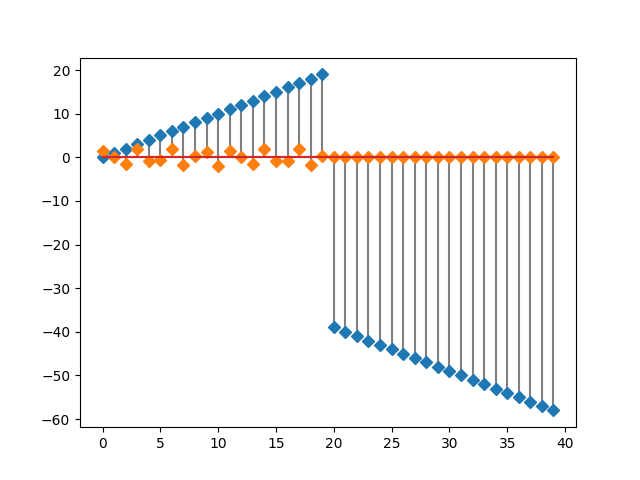
\includegraphics[width=0.7\textwidth]{figures/zad1_signali.png}
        \end{center}
    
    \item Prikaz rezultata linearne konvolucije i rezulata funkcije \textit{conv}
    	
        \begin{center}
            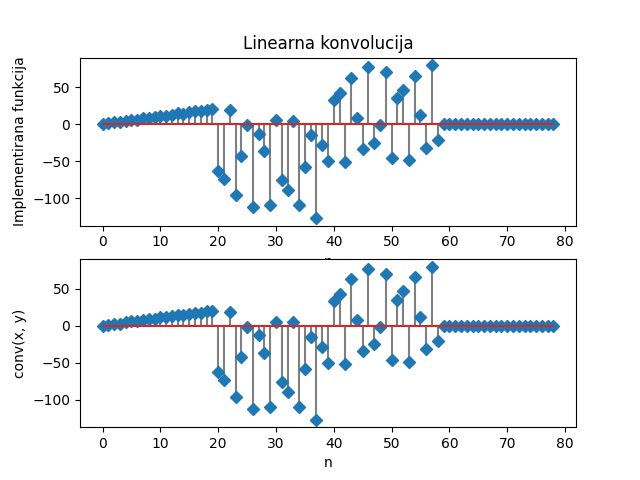
\includegraphics[width=0.7\textwidth]{figures/zad1_linearna_konvolucija.png}
        \end{center}
        
    \item Prikaz rezultata ciklične konvolucije i rezulata funkcije \textit{cconv}
    
        \begin{center}
            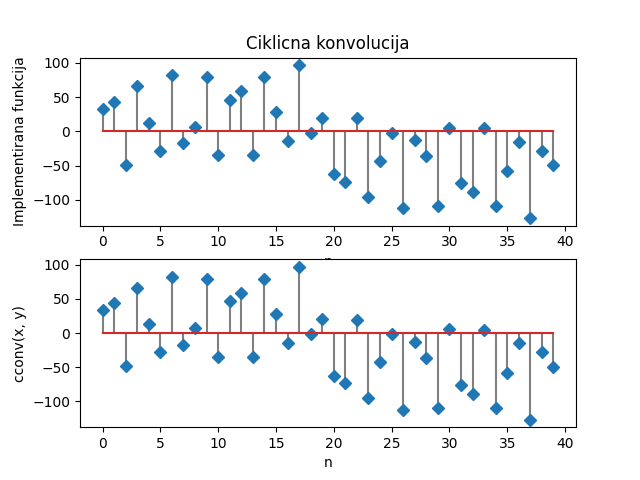
\includegraphics[width=0.7\textwidth]{figures/zad1_ciklicna_konvolucija_provera.png}
        \end{center}
        

    \item Linearna i ciklična konvolucija imaju iste vrednosti u sledećim odbircima
    
        \begin{center}
            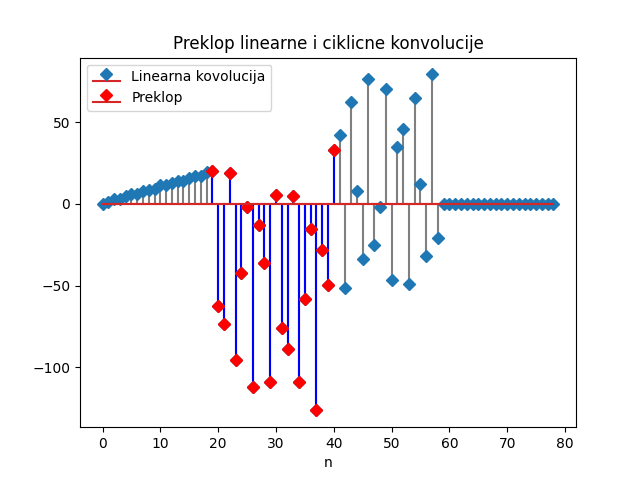
\includegraphics[width=0.7\textwidth]{figures/zad1_overlap.png}
        \end{center}
    
    \item{Programski k\^{o}d}
    \lstinputlisting[language=Python]{code/zad1.py}
  
\end{itemize}

